\documentclass[border=4pt]{standalone}

\usepackage{amsmath}
\usepackage{tikz}
\usepackage{mathdots}
\usepackage{yhmath}
\usepackage{cancel}
\usepackage{color}
\usepackage{siunitx}
\usepackage{array}
\usepackage{multirow}
\usepackage{amssymb}
\usepackage{gensymb}
\usepackage{tabularx}
\usepackage{booktabs}
\usetikzlibrary{fadings}
\usetikzlibrary{patterns}


\begin{document}


\tikzset{every picture/.style={line width=0.75pt}} %set default line width to 0.75pt        

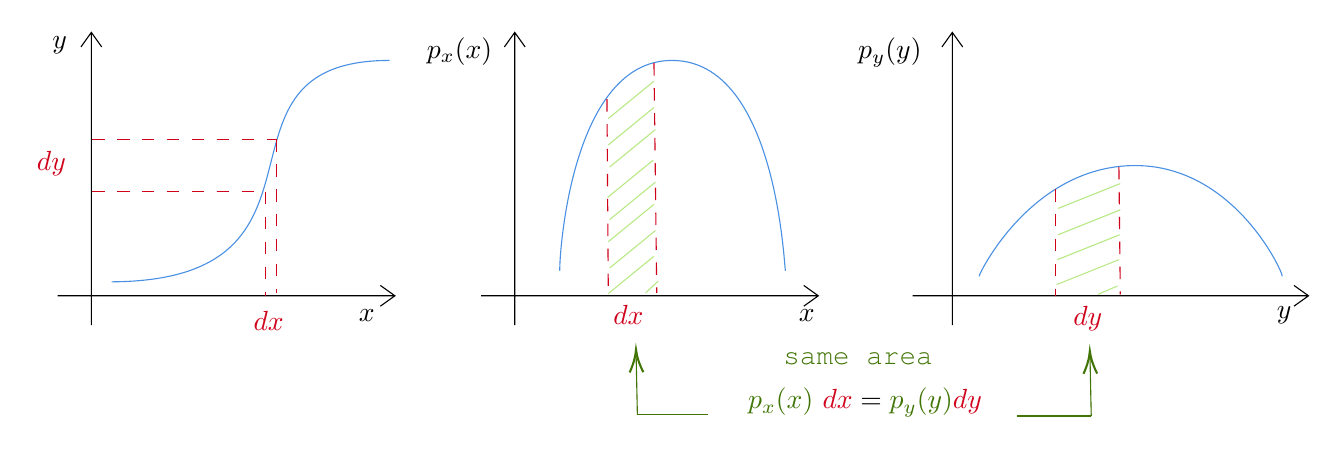
\begin{tikzpicture}[x=0.75pt,y=0.75pt,yscale=-1,xscale=1]
%uncomment if require: \path (0,489); %set diagram left start at 0, and has height of 489

%Shape: Axis 2D [id:dp8395468765016407] 
\draw  (25,189.9) -- (187.5,189.9)(41.25,63) -- (41.25,204) (180.5,184.9) -- (187.5,189.9) -- (180.5,194.9) (36.25,70) -- (41.25,63) -- (46.25,70)  ;
%Shape: Axis 2D [id:dp03103253266522432] 
\draw  (229,189.9) -- (391.5,189.9)(245.25,63) -- (245.25,204) (384.5,184.9) -- (391.5,189.9) -- (384.5,194.9) (240.25,70) -- (245.25,63) -- (250.25,70)  ;
%Shape: Axis 2D [id:dp87656515098485] 
\draw  (437,189.9) -- (627.67,189.9)(456.07,63) -- (456.07,204) (620.67,184.9) -- (627.67,189.9) -- (620.67,194.9) (451.07,70) -- (456.07,63) -- (461.07,70)  ;
%Curve Lines [id:da9113299974490501] 
\draw [color={rgb, 255:red, 74; green, 144; blue, 226 }  ,draw opacity=1 ]   (51,183.17) .. controls (169,182.5) and (90.33,76.5) .. (185,76.5) ;
%Straight Lines [id:da9834597587142864] 
\draw [color={rgb, 255:red, 208; green, 2; blue, 27 }  ,draw opacity=1 ] [dash pattern={on 4.5pt off 4.5pt}]  (41.67,114.5) -- (130.33,114.5) ;
%Straight Lines [id:da0005008593628319513] 
\draw [color={rgb, 255:red, 208; green, 2; blue, 27 }  ,draw opacity=1 ] [dash pattern={on 4.5pt off 4.5pt}]  (41.67,139.83) -- (125,139.83) ;
%Straight Lines [id:da7892221405741688] 
\draw [color={rgb, 255:red, 208; green, 2; blue, 27 }  ,draw opacity=1 ] [dash pattern={on 4.5pt off 4.5pt}]  (130.33,114.5) -- (130.33,188.5) ;
%Straight Lines [id:da2207214368548256] 
\draw [color={rgb, 255:red, 208; green, 2; blue, 27 }  ,draw opacity=1 ] [dash pattern={on 4.5pt off 4.5pt}]  (125,139.83) -- (125,189.83) ;
%Curve Lines [id:da6711029390119463] 
\draw [color={rgb, 255:red, 74; green, 144; blue, 226 }  ,draw opacity=1 ]   (267,177.83) .. controls (266.33,178.5) and (270.33,76.5) .. (321,76.5) .. controls (371.67,76.5) and (375,176.5) .. (375.67,177.83) ;
%Straight Lines [id:da9551736816076641] 
\draw [color={rgb, 255:red, 208; green, 2; blue, 27 }  ,draw opacity=1 ] [dash pattern={on 4.5pt off 4.5pt}]  (312.33,77.83) -- (313.67,188.5) ;
%Straight Lines [id:da4355379591655777] 
\draw [color={rgb, 255:red, 208; green, 2; blue, 27 }  ,draw opacity=1 ] [dash pattern={on 4.5pt off 4.5pt}]  (289.67,95.17) -- (290.33,189.83) ;
%Curve Lines [id:da07850694147964132] 
\draw [color={rgb, 255:red, 74; green, 144; blue, 226 }  ,draw opacity=1 ]   (469,180.5) .. controls (468.33,180.5) and (493,128.5) .. (542.33,127.17) .. controls (591.67,125.83) and (615.67,179.17) .. (615,180.5) ;
%Straight Lines [id:da3774128108157011] 
\draw [color={rgb, 255:red, 208; green, 2; blue, 27 }  ,draw opacity=1 ] [dash pattern={on 4.5pt off 4.5pt}]  (536.33,127.83) -- (537,189.17) ;
%Straight Lines [id:da9777846608473144] 
\draw [color={rgb, 255:red, 208; green, 2; blue, 27 }  ,draw opacity=1 ] [dash pattern={on 4.5pt off 4.5pt}]  (505.67,138.5) -- (505.67,189.83) ;
%Straight Lines [id:da722976060336801] 
\draw [color={rgb, 255:red, 184; green, 233; blue, 134 }  ,draw opacity=1 ]   (290.33,117.17) -- (312.33,99.17) ;
%Straight Lines [id:da7399996019241906] 
\draw [color={rgb, 255:red, 184; green, 233; blue, 134 }  ,draw opacity=1 ]   (290,142.5) -- (312,124.5) ;
%Straight Lines [id:da7774301381655364] 
\draw [color={rgb, 255:red, 184; green, 233; blue, 134 }  ,draw opacity=1 ]   (290.33,163.83) -- (312.33,145.83) ;
%Straight Lines [id:da45360694816447444] 
\draw [color={rgb, 255:red, 184; green, 233; blue, 134 }  ,draw opacity=1 ]   (290.33,104.5) -- (312.33,86.5) ;
%Straight Lines [id:da8794171407300717] 
\draw [color={rgb, 255:red, 184; green, 233; blue, 134 }  ,draw opacity=1 ]   (291,127.83) -- (313,109.83) ;
%Straight Lines [id:da31741837946963325] 
\draw [color={rgb, 255:red, 184; green, 233; blue, 134 }  ,draw opacity=1 ]   (291,153.17) -- (313,135.17) ;
%Straight Lines [id:da2501525496500008] 
\draw [color={rgb, 255:red, 184; green, 233; blue, 134 }  ,draw opacity=1 ]   (291,176.5) -- (313,158.5) ;
%Straight Lines [id:da581003620032698] 
\draw [color={rgb, 255:red, 184; green, 233; blue, 134 }  ,draw opacity=1 ]   (290.33,188.83) -- (312.33,170.83) ;
%Straight Lines [id:da3973067222256279] 
\draw [color={rgb, 255:red, 184; green, 233; blue, 134 }  ,draw opacity=1 ]   (507,147.83) -- (537,135.83) ;
%Straight Lines [id:da2559364125548371] 
\draw [color={rgb, 255:red, 184; green, 233; blue, 134 }  ,draw opacity=1 ]   (507,160.5) -- (537,148.5) ;
%Straight Lines [id:da40056262468791703] 
\draw [color={rgb, 255:red, 184; green, 233; blue, 134 }  ,draw opacity=1 ]   (506.67,172.5) -- (536.67,160.5) ;
%Straight Lines [id:da4953169570590341] 
\draw [color={rgb, 255:red, 184; green, 233; blue, 134 }  ,draw opacity=1 ]   (506.33,184.5) -- (536.33,172.5) ;
%Straight Lines [id:da7083537186918716] 
\draw [color={rgb, 255:red, 184; green, 233; blue, 134 }  ,draw opacity=1 ]   (526.33,189.17) -- (535.67,185.17) ;
%Straight Lines [id:da5222442690670956] 
\draw [color={rgb, 255:red, 184; green, 233; blue, 134 }  ,draw opacity=1 ]   (308.33,188.5) -- (314.33,182.83) ;
%Straight Lines [id:da29648012627628817] 
\draw [color={rgb, 255:red, 65; green, 117; blue, 5 }  ,draw opacity=1 ]   (304.33,247.17) -- (303.71,217.83) ;
\draw [shift={(303.67,215.83)}, rotate = 448.78] [color={rgb, 255:red, 65; green, 117; blue, 5 }  ,draw opacity=1 ][line width=0.75]    (10.93,-3.29) .. controls (6.95,-1.4) and (3.31,-0.3) .. (0,0) .. controls (3.31,0.3) and (6.95,1.4) .. (10.93,3.29)   ;
%Straight Lines [id:da703733746911102] 
\draw [color={rgb, 255:red, 65; green, 117; blue, 5 }  ,draw opacity=1 ][fill={rgb, 255:red, 65; green, 117; blue, 5 }  ,fill opacity=1 ]   (523,247.83) -- (522.38,218.5) ;
\draw [shift={(522.33,216.5)}, rotate = 448.78] [color={rgb, 255:red, 65; green, 117; blue, 5 }  ,draw opacity=1 ][line width=0.75]    (10.93,-3.29) .. controls (6.95,-1.4) and (3.31,-0.3) .. (0,0) .. controls (3.31,0.3) and (6.95,1.4) .. (10.93,3.29)   ;
%Straight Lines [id:da8213901818676554] 
\draw [color={rgb, 255:red, 65; green, 117; blue, 5 }  ,draw opacity=1 ][fill={rgb, 255:red, 65; green, 117; blue, 5 }  ,fill opacity=1 ]   (304.33,247.17) -- (338.33,247.17) ;
%Straight Lines [id:da9096701558080469] 
\draw [color={rgb, 255:red, 65; green, 117; blue, 5 }  ,draw opacity=1 ][fill={rgb, 255:red, 65; green, 117; blue, 5 }  ,fill opacity=1 ]   (487,247.83) -- (523,247.83) ;

% Text Node
\draw (126.67,202) node  [color={rgb, 255:red, 208; green, 2; blue, 27 }  ,opacity=1 ]  {$dx$};
% Text Node
\draw (22,126) node  [color={rgb, 255:red, 208; green, 2; blue, 27 }  ,opacity=1 ]  {$dy$};
% Text Node
\draw (300,199.33) node  [color={rgb, 255:red, 208; green, 2; blue, 27 }  ,opacity=1 ]  {$dx$};
% Text Node
\draw (521.33,201) node  [color={rgb, 255:red, 208; green, 2; blue, 27 }  ,opacity=1 ]  {$dy$};
% Text Node
\draw (414,241.33) node    {$\textcolor[rgb]{0.25,0.46,0.02}{p_{x}( x)} \ \textcolor[rgb]{0.82,0.01,0.11}{dx} =\textcolor[rgb]{0.25,0.46,0.02}{p_{y}( y)}\textcolor[rgb]{0.82,0.01,0.11}{dy}$};
% Text Node
\draw (410.67,220) node  [color={rgb, 255:red, 65; green, 117; blue, 5 }  ,opacity=1 ] [align=left] {{\fontfamily{pcr}\selectfont same area}};
% Text Node
\draw (26,69.33) node    {$y$};
% Text Node
\draw (174,199.33) node    {$x$};
% Text Node
\draw (386,199.33) node    {$x$};
% Text Node
\draw (616,199.33) node    {$y$};
% Text Node
\draw (218.67,72) node    {$p_{x}( x)$};
% Text Node
\draw (426,72.67) node    {$p_{y}( y)$};


\end{tikzpicture}

\end{document}
